\section{Analyse de l'existant}

Actuellement le savoir-faire est très limité, en effet il y a peu de processus de gestion déclenchés pour surveiller les sites. Le schéma ci-dessous résume la surveillance actuelle.

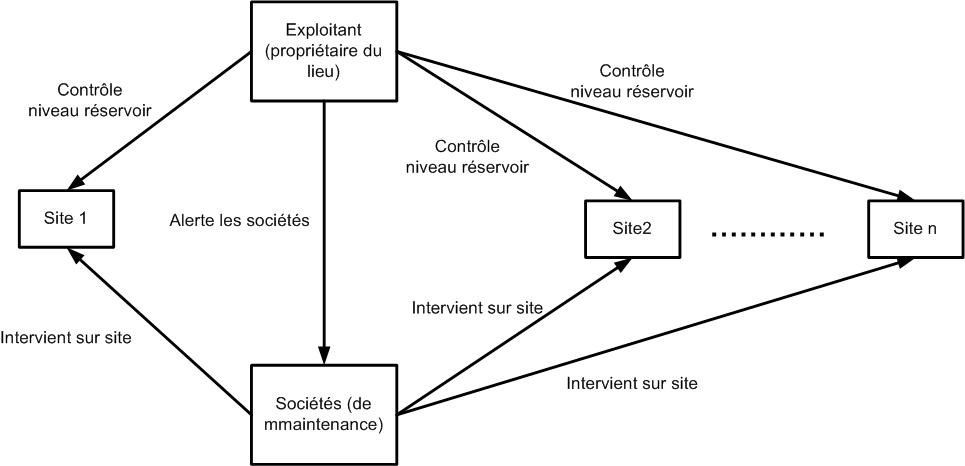
\includegraphics[width=0.9\textwidth]{img/schemaAnalyseExistant.png}

Le matériel est celui utilisé par les sociétés de maintenance intervenant sur les sites (camions, systèmes de vidage/remplissage..)
Deux métiers ont été identifiés, les propriétaires des sites s’occupent de leur exploitation tandis que les sociétés spécialisés sont chargées du métier de la maintenance.
